% \clearpage
% \subsection{\label{Run14TPC_YF}Run11 TPC analysis YF}

\newcommand{\ttbs}{\char'134}
% \newcommand{\AmS}{{\protect\the\textfont2A\kern-.1667em\lower.5ex\hbox{M}\kern-.125emS}}
\hyphenation{author another created financial paper re-commend-ed}
\newcommand{\pt}{$p_{T}$ }
\newcommand{ \bfg }{\begin{figure}[]}
\newcommand{ \efg }{\end{figure}}
\newcommand{\dzero}{$D^{0}$ }



%%%%%%%%%%%%%%%%%%%%%%%%%%%%%%%%%%%%%%%%%%%%%%%%%%
%                                                %
%    BEGINNING OF TEXT                           %
%                                                %
%%%%%%%%%%%%%%%%%%%%%%%%%%%%%%%%%%%%%%%%%%%%%%%%%%

Since at \pt\ $<$ 2 GeV/$c$ a discrepancy was found between new data from Run14 with HFT and published data from Run10+Run11. A re-analysis on Run11 data was performed to check if anything was incorrect. The analysis cuts are the same as in previous analysis note:

https://drupal.star.bnl.gov/STAR/system/files/dzeroAuAu$\_$updated.pdf

also listed in Xiaolong 's analysis, see next section. The only difference is varying DCA cut with $<$ 1 cm or $<$ 2 cm.

The raw signals as a function of \pt\ from part of Run11 data with 85\% of full statistics were extracted as Fig.\ref{D0inpt1},

\bfg \centering
%\vspace{-0.2in}
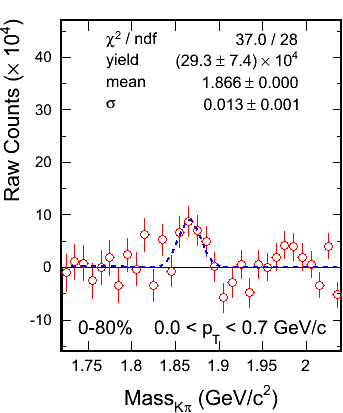
\includegraphics[width=0.3\textwidth]{figure/Run11_YF/D0_0-80_1_7_signal.png}
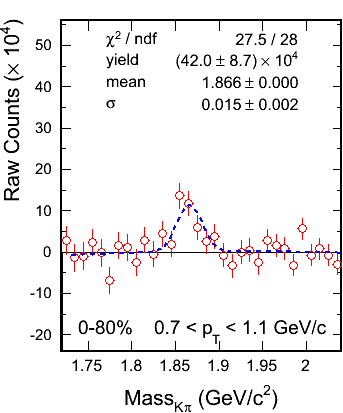
\includegraphics[width=0.3\textwidth]{figure/Run11_YF/D0_0-80_8_11_signal.png}
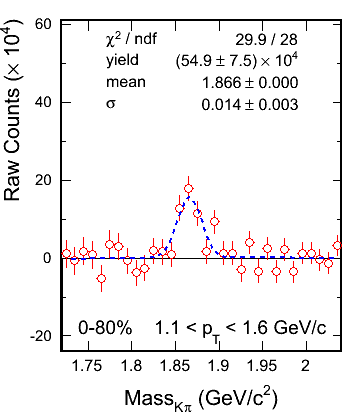
\includegraphics[width=0.3\textwidth]{figure/Run11_YF/D0_0-80_12_16_signal.png}
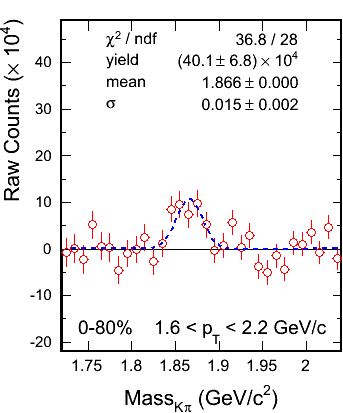
\includegraphics[width=0.3\textwidth]{figure/Run11_YF/D0_0-80_17_22_signal.png}
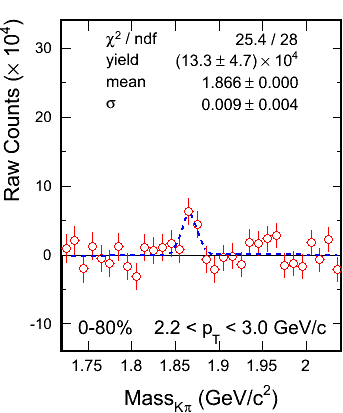
\includegraphics[width=0.3\textwidth]{figure/Run11_YF/D0_0-80_23_30_signal.png}
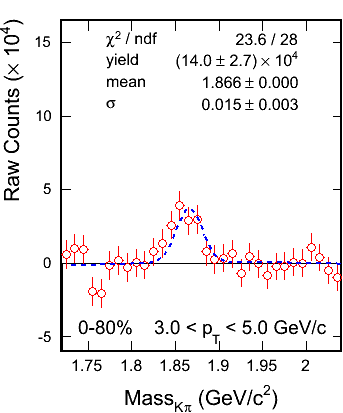
\includegraphics[width=0.3\textwidth]{figure/Run11_YF/D0_0-80_31_50_signal.png}
%\vspace{+0.2in}
\caption{\pt\ dependence of \dzero\ signals in 0-80\% from partial Run11 data.}
\label{D0inpt1}
\efg

The raw signals were compared with Xiaolong 's independent analysis and found to be consistent, shown in Fig.\ref{rawsig}. The slight lower yield in Xiaolong 's analysis is due to the tight DCA cut $<$ 1 cm, while the DCA cut applied here is $<$ 2 cm.

\bfg \centering
%\vspace{-0.2in}
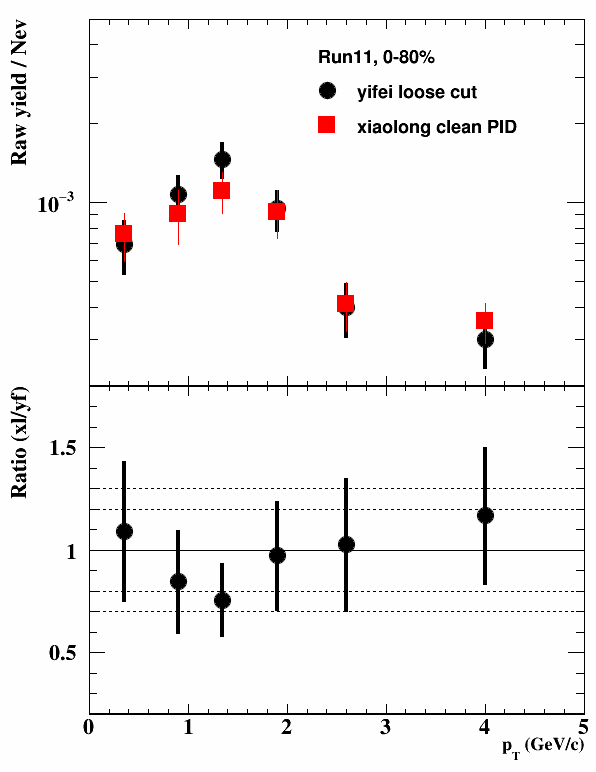
\includegraphics[width=0.6\textwidth]{figure/Run11_YF/RawY_0_80.png}
\caption{Raw signals comparison with Xiaolong 's.}
\label{rawsig}
\efg

In early days, there was no vertex detector, we had to use random combination of decay products to reconstruct \dzero\ meson in hadronic channel, which suffered from huge combinatorial background. The way to improve the significance was to enrich the kaon and pion PID probability and enhance the statistics as much as possible at the same time. Thus we developed a hybrid method: In low momentum region, we always required good TOF matching and TOF PID, those tracks without good TOF matching or failed to pass TOF PID were rejected. In high momentum region, it is the same as low momentum, but for those tracks without TOF matching or failed to pass TOF PID, we still kept them and use TPC PID to enhance the statistics, since TOF helps little for high momentum tracks. The details are list below:

A good TOF matching means tracks satisfy TOFMatchFlag $>$ 0 \&\& beta $>$ 0.

At low momentum, p $<$ 1.6 GeV/c, the correct algorithm to ensure the purity of kaons and pions is:

GoodTOFMatching \&\& TPC PID \&\& TOF PID (see Eq. 23 - 25)

At high momentum, p $>$ 1.6 GeV/c , if there was a good TOF matching, we applied TPC PID + TOF PID, otherwise we used TPC PID only  to enhance the PID efficiency:

If (GoodTOFMatching) TPC PID + TOF PID
else TPC PID

But an issue was found in the code, that the condition to reject those tracks without matching to TOF at low momentum was different from above algorithm and also different from what we used to calculate the efficiency. We found that those tracks with TOFMatchFlag $>$ 0 but with beta $<$ 0 were not correctly rejected, which results in higher yield obtained or lower efficiency than expected. This introduces about 15\% difference at low \pt\ but does not affect high \pt much.

\bfg \centering
%\vspace{-0.2in}
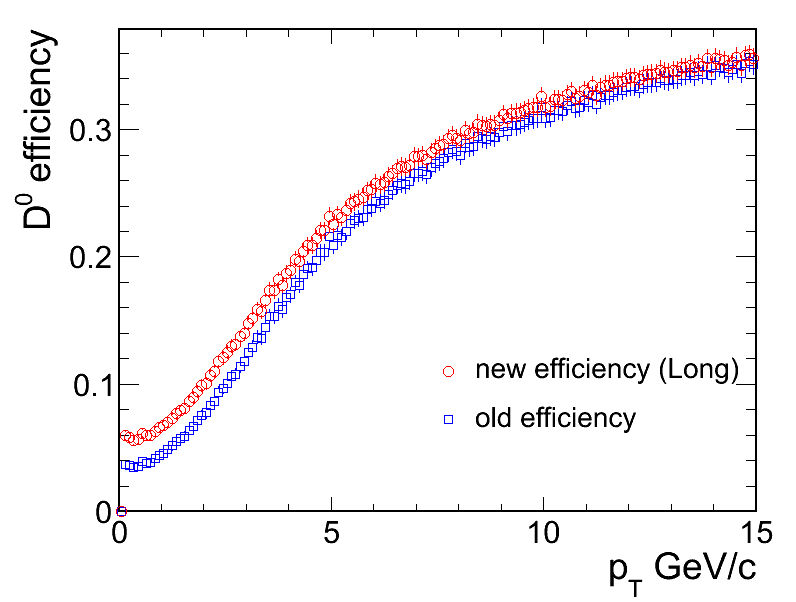
\includegraphics[width=0.6\textwidth]{figure/Run11_YF/eff.png}
\caption{New efficiency checked from Long compared with old one.}
\label{effnew}
\efg

The other issue is that we applied an additional $DCA_{XY}$ cut efficiency in previous analysis. This cut was used in TOF matching algorithm (in TOFMatchMaker) to require tracks with a distance of closest approach to the beam line in xy plane within 1 cm. This efficiency was studied in early days and found there was about up to 20\% of tracks at low \pt\ rejected with this cut, see Fig.\ref{DCAxyeff}. However, when we studied TOF matching efficiency, we used a data driven method and this efficiency should be already included. Thus we double counting this efficiency.

\bfg \centering
%\vspace{-0.2in}
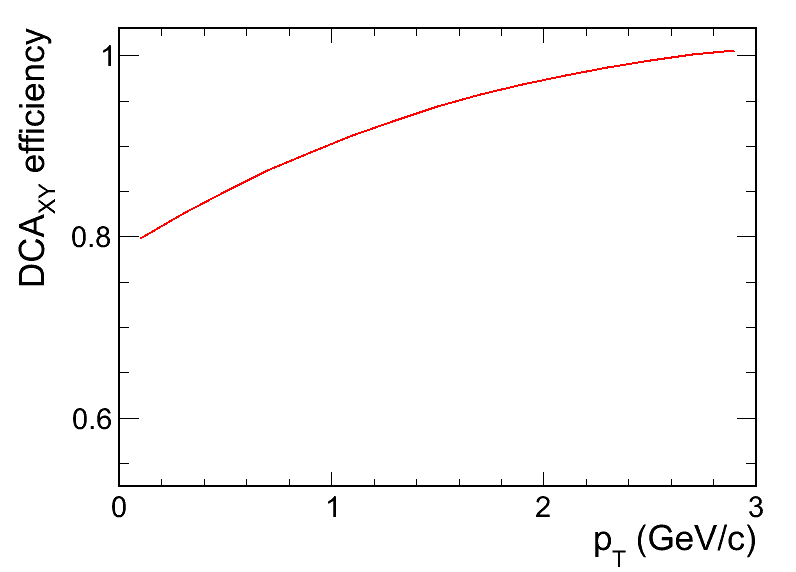
\includegraphics[width=0.6\textwidth]{figure/Run11_YF/DCAxyEff.png}
\caption{$DCA_{XY}$ efficiency.}
\label{DCAxyeff}
\efg

\subsubsection{Added by Long Zhou}
After corrected above two main issues, the corrected reconstruction efficiency can be found at Fig.\ref{RecEff}

\bfg \centering
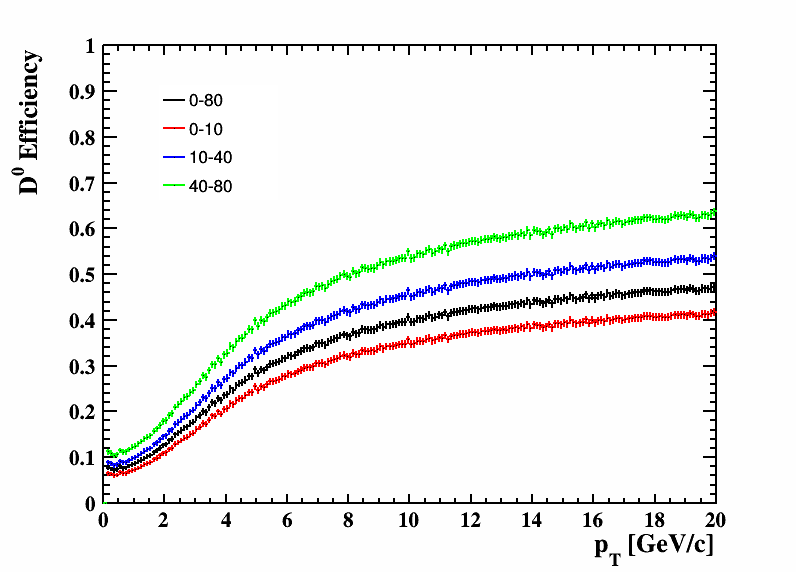
\includegraphics[width=0.6\textwidth]{figure/Run11_YF/rec_eff.png}
\caption{The reconstruction efficiency at each centrality bin}
\label{RecEff}
\efg

% Add the re-produced spectra and R_AA 


The final $D^0$ $R_{AA}$ spectra will corrected by efficiency ratio between the published reconstruction efficiency and the corrected reconstruction efficiency. The  corrected $D^0$ $R_{AA}$ is  shown in Fig.\ref{CorRaa}

\bfg \centering
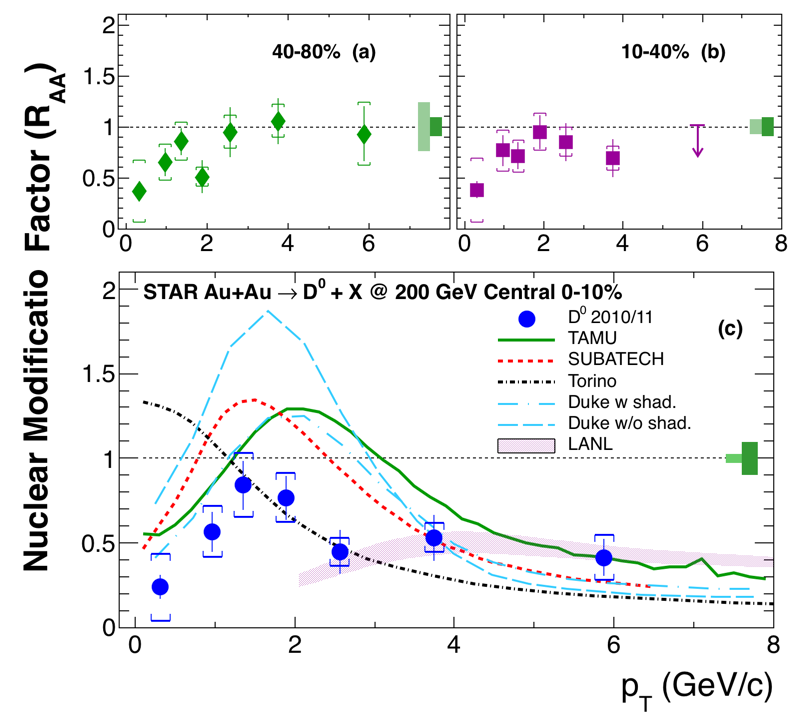
\includegraphics[width=0.8\textwidth]{figure/Run11_YF/fig3.png}
\caption{The Corrected $D^0$ $R_{AA}$ in each centrality class, and compared with several model calculation }
\label{CorRaa}
\efg

The updated $D^0$ $R_{AA}$ was also compared to the previous results, shown in Fig.\ref{CorRaa33}. As can clear see the difference in the middle transverse momentum range.

\bfg \centering
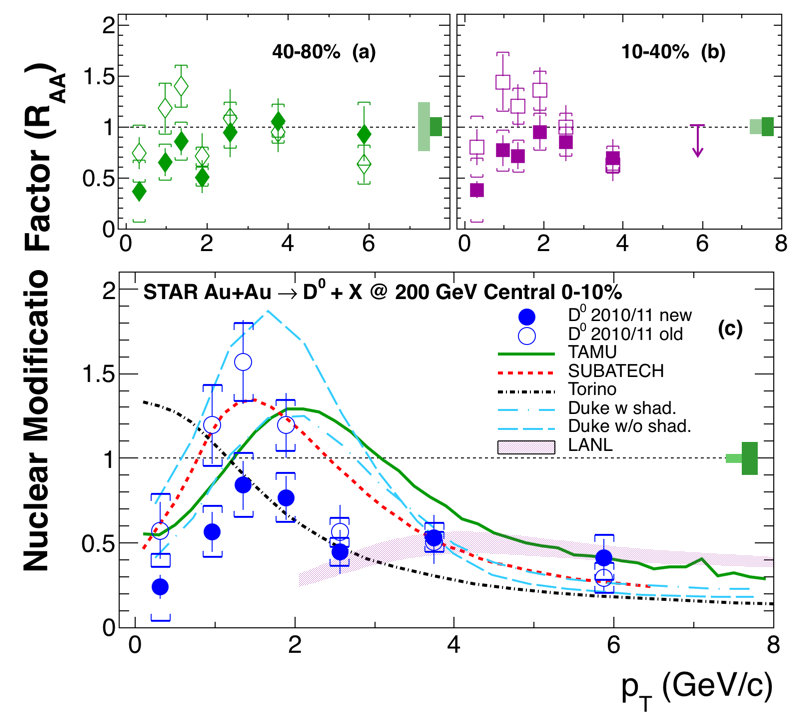
\includegraphics[width=0.8\textwidth]{figure/Run11_YF/fig33.png}
\caption{The Corrected $D^0$ $R_{AA}$ in each centrality class, and compared with several model calculation, also compared to the previous publish results.}
\label{CorRaa33}
\efg

\emph{Need the $R_{AA}$ comparison plots between my $R_{AA}$  and Run 14 $R_{AA}$(from Xiaolong) }

More material can be found at here :  
\\https://drupal.star.bnl.gov/STAR/system/files/D0\_Eff\_discussion\_2016\_11\_7.pdf
\\https://drupal.star.bnl.gov/STAR/system/files/D0\_Eff\_discussion\_2017\_05\_12.pdf
\\https://drupal.star.bnl.gov/STAR/system/files/D0\_BNL170516\_0.pdf
% \end{document}


%%%%%%%%%%%%%%%%%%%%%%
% End of tex  %
%%%%%%%%%%%%%%%%%%%%%%

